%% ****** Start of file aiptemplate.tex ****** %
%%
%%   This file is part of the files in the distribution of AIP substyles for REVTeX4.
%%   Version 4.1 of 9 October 2009.
%%
%
% This is a template for producing documents for use with 
% the REVTEX 4.1 document class and the AIP substyles.
% 
% Copy this file to another name and then work on that file.
% That way, you always have this original template file to use.

%\documentclass[aip,graphicx]{revtex4-1}
%\documentclass[aip,reprint]{revtex4-1}

%\usepackage{graphicx}

%\draft % marks overfull lines with a black rule on the right
\documentclass[pre,aps,floatfix,authordate1-4,twocolumn]{revtex4-1}
%\documentclass[pre,aps,floatfix,authordate1-4]{revtex4-1}

%\documentclass[aps,prl,preprint,superscriptaddress]{revtex4}



%\documentclass[aps,prl,preprint,groupedaddress]{revtex4}

\usepackage{rotating} 
\usepackage{times}
\usepackage{graphicx}
\usepackage{setspace}
\usepackage{amsmath}
\usepackage{epstopdf}
\usepackage[obeyFinal]{easy-todo}
\begin{document}

% Use the \preprint command to place your local institutional report number 
% on the title page in preprint mode.
% Multiple \preprint commands are allowed.
%\preprint{}

\title{Rotational dynamics of proteins from spin relaxation rates and molecular dynamics simulations} %Title of paper

% repeat the \author .. \affiliation  etc. as needed
% \email, \thanks, \homepage, \altaffiliation all apply to the current author.
% Explanatory text should go in the []'s, 
% actual e-mail address or url should go in the {}'s for \email and \homepage.
% Please use the appropriate macro for the type of information

% \affiliation command applies to all authors since the last \affiliation command. 
% The \affiliation command should follow the other information.

\author{O. H. Samuli Ollila}
\email[]{samuli.ollila@helsinki.fi}
%\homepage[]{Your web page}
%\thanks{}
\altaffiliation{Department of Neuroscience and Biomedical Engineering, Aalto University}
\affiliation{Insititute of Biotechnology, University of Helsinki}

% Collaboration name, if desired (requires use of superscriptaddress option in \documentclass). 
% \noaffiliation is required (may also be used with the \author command).
%\collaboration{}
%\noaffiliation

\date{\today}

\begin{abstract}
  % insert abstract here
  
\end{abstract}

%\pacs{}% insert suggested PACS numbers in braces on next line

\maketitle %\maketitle must follow title, authors, abstract and \pacs

% Body of paper goes here. Use proper sectioning commands. 
% References should be done using the \cite, \ref, and \label commands


%\label{}
\section{Introduction}
Spin relaxation rates measured with NMR techniques give segmental resolution
information about rotational dynamics of proteins and macromolecules.
Various models have been used to separate internal dynamics and order from
overall rotational diffusion of molecules \cite{??}.
These techniques have been highly useful in characterization of 
rotational diffusion and internal flexibility of proteins and other biomolecules.
On the other hand, segmental level information has been used in validation
and improvement of molecular dynamics simulation force fields \cite{??}.
Segmental order has been also related to conformational entropy of proteins \cite{??}.

Spin relaxation rates are typically intepreted by using various dynamical models
assuming different level of complexity of rotational relaxation processes.
The most simplistic models assume single timescale and order parameter for internal
motion and isotropic overall rotational diffusion. However, biomolecules often experience
anisotropic overall diffusion and several internal timescales. Models for more complicated
models have been also introduced, however, there are more fitting parameters in these models
and intepretation of experiments becomes extensively difficult.

Classical molecular dynamics simuations contain, in principle, all the complexity of the
timescales and could be used to interpret the rotational dynamics measured with spin
relaxation experiments. However, this has not been a trivial task due to the force field
issues and limited available time scales in the simulations.

In this work we present approach that can be used to analyze spin relaxation experiments
by using classical molecular dynamics simulations. The approach can be used for anisotropic
molecules and allows a correction of anisotropic overall diffusion. We demonstrate
the usage of the approach for two aniotropic protein constructs from engineered from
Helicobacteri pyroli and Pseudomonas.


\section{Methods}

\subsection{Spin relaxation and rotational dynamics of molecules}

Spin relaxation rates $R_1$, $R_2$ and $R_{\rm NOE}$ measured from NMR experiments
for N-H bondsare related to the molecular dynamics through spectral density $J(\omega)$ and equations \cite{abragam,kay89}
\begin{equation}\label{R1}
  \begin{aligned}
  R_{1}= & \frac{d_{\rm{NH}}^2N_{\rm{H}}}{20}\bigg[J(\omega_{\rm{H}}-\omega_{\rm{N}})+3J(\omega_{\rm{N}})+6J(\omega_{\rm{N}}+\omega_{\rm{H}})\bigg] \\
        & +\frac{(\sigma \omega_{\rm{N}})^2}{15}j(\omega_{\rm{N}}),
  \end{aligned}
\end{equation}
\begin{equation}\label{R2}
    \begin{aligned}
  R_{2}= & \frac{1}{2}\frac{d_{\rm{NH}}^2N_{\rm{H}}}{20}\bigg[4J(0)+3j(\omega_{\rm{N}})+J(\omega_{\rm{H}}-\omega_{\rm{N}})+6J(\omega_{\rm{H}})  \\
    & +6J(\omega_{\rm{N}}+\omega_{\rm{H}})\bigg]+\frac{(\sigma \omega_{\rm{N}})^2}{15*6}[4J(0) +3J(\omega_{\rm{N}})],
    \end{aligned}
\end{equation}
\begin{equation}\label{NOE}
R_{\rm NOE}=1+\frac{d_{\rm{NH}}^2N_{\rm{H}}}{20}\bigg[6J(\omega_{\rm{N}}+\omega_{\rm{H}})+J(\omega_{\rm{H}}-\omega_{\rm{N}}))\bigg]\frac{\gamma_{\rm{H}}}{\gamma_{\rm{N}}R_1},
\end{equation}
where $\omega_{\rm{N}}$ and $\omega_{\rm{H}}$ are the Larmor angular frequencies of $^{15}$N and $^1$H respectively,
$N_{\rm{H}}$ is the number of bound protons. The dipolar coupling constant is given by
\begin{equation}
d_{\rm{NH}}=-\frac{\mu_0\hbar\gamma_{\rm{H}}\gamma_{\rm{N}}}{4\pi\langle r_{\rm{CN}}^3\rangle},\nonumber
\end{equation}
where $\mu_0$ is the magnetic constant or vacuum permeability, $\hbar$ is the reduced Planck constant,
$\gamma_{\rm{N}}$ and $\gamma_{\rm{H}}$ are the gyromagnetic constants of $^{15}$N and $^1$H, respectively.
Average cubic length is $\langle r_{\rm{CN}}^3\rangle \approx$ and the 
chemical shift anisotropy is $\Delta \sigma \approx 160*10^{-6}$ for N-H bonds in proteins \cite{??}.

Spectral density $J(\omega)$ is the Fourier transformation of the second order
rotational correlation function for N-H bond
\begin{equation}\label{SPECTdens}
  J(\omega)=2\int_0^\infty C(t) \cos(\omega t) {\rm d}t.
\end{equation}
The second order rotational correlation is defined as
\begin{equation}\label{CORRFdef}
  C(t)=\langle (3\cos^2\theta_{t';t'+t}-1)/2 \rangle_{t'},
\end{equation}
where average is ensemble average and $\theta$ is the angle between N-H bonds at times $t'$ and $t'+t$.
The rotational correlation function for protein tumbling in solution
contains information about overall rotation of the molecule as well as
internal relaxation processes. Assuming that these are independent,
the rotational correlation function can be written as \cite{??}
\begin{equation}\label{CORRFsep}
  C(t)=C_I(t)C_O(t),
\end{equation}
where $C_I(t)$ and $C_O(t)$ are correlation functions for internal and overall
rotiations, respectively. Correlation function for fully anisotropic overall
rotation can be written as a sum of five exponentials \cite{??}
\begin{equation}\label{CORRFanisot}
  C_O(t)=\sum_{j=1}^5 A_j e^{-t/\tau_j},
\end{equation}
where time constants $\tau_j$ are related \footnote{
$\tau_1=(4D_{xx}+D_{yy}+D_{zz})^{-1}$,
$\tau_2=(D_{xx}+4D_{yy}+D_{zz})^{-1}$,
$\tau_3=(D_{xx}+D_{yy}+4D_{zz})^{-1}$,
$\tau_4=[6(D+(D^2-L^2)^{-1/2}]^{-1}$,
$\tau_5=[6(D-(D^2-L^2)^{-1/2}]^{-1}$,
$D=\frac{1}{3}(D_{xx}+D_{yy}+D_{zz})$ and 
$L^2=\frac{1}{3}(D_{xx}D_{yy}+D_{xx}D_{zz}+D_{yy}D_{zz})$} to
the diffusion constants around
three principal axes of a molecule
$D_{xx}$, $D_{yy}$ and $D_{zz}$,  
defined as 
\begin{equation}\label{DIFFdef}
  \begin{aligned}
    \langle (\Delta \alpha_{t';t'+t})^2 \rangle_{t'} = 2 D_{xx} t \\
    \langle (\Delta \beta_{t';t'+t})^2 \rangle_{t'} = 2 D_{yy} t \\
    \langle (\Delta \gamma_{t';t'+t})^2 \rangle_{t'} = 2 D_{zz} t, \\
  \end{aligned}
\end{equation}
where $\langle (\Delta \alpha_{t';t'+t})^2 \rangle_{t'}$,
$\langle (\Delta \beta_{t';t'+t})^2 \rangle_{t'}$ and
$\langle (\Delta \gamma_{t';t'+t})^2 \rangle_{t'}$ are mean
square angle deviations of protein intertia axes.
%\begin{equation}
%  C'_I(t)= e^{-t/\tau_c},
%\end{equation}
The internal correlation function decays to a plateau, which
defines the square of order parameter respect to molecular axes $S^2$.
The effective internal correlation time can be defined with the
help of reduced correlation function $C_I'(t)=(C_I-S^2)/(1-S^2)$ \cite{??}
\begin{equation}
  \tau_{\rm eff}=\int_0^\infty C_I'(t) \mathrm{d}t.
\end{equation}

Standard analyses of experimental relaxation data usually assume
fully or axially isotropic overall rotational motion and single
decay constant for interal motion. Then the free parameters
($S^2$, $\tau_j$, $A_j$) are fit against spin relaxation data
from experiments. This gives most likely very good results for
isotropic molecules for which the assumption of single internal
motional timescale is reasonable. However, for molecules with
significant shape anisotropy or several timescales in internal
motions the amoount parameters to be fitted becomes large compared
with the typical amount of experimental points.

\subsection{Rotational dynamics from molecular dynamics simulations}\label{MDanalysis}
Classical molecular dynamics simulations give trajectories of individual
atoms as a function of time, which can be used to calculate rotational
correlation functions for each bond and explicit separation of internal
and overall rotational motions of molecules. The rotational
correlation functions can be used to calculate spin relaxation times
through Eqs. \ref{T1}-\ref{SPECdens}, which can be then compared to the
experimental data in order to assess simulation model quality \cite{??} and interpret
experiments \cite{??}. However, the comparison is often complicated by
the short simulation times \cite{??} and incorrect overall rotational
diffusion due to water models \cite{??}. These issues have been typically
overcame by introducing isotropic rotational diffusion term in the correlation
functions \cite{??} or comparing order parameters instead of spin relaxation rates \cite{??}.
These approaches are not, however, useful for anitropic proteins and order
parameter comparison is not direct comparison between simulations and experiments in
the case of freely rotating molecules. 

Method presented here can be applied also to anisotropic proteins simulated
with timescales routinely accessible with state of the art computational
infrastructure. The key idea of the method is to calculate the rotational
diffusion constants and then use Eq. \ref{CORRFanisot} to determine the
correlation function related to the overall rotational diffusion. 

Here we present method to analyse rotational dynamics,
The analysis of rotational dynamics permormed in this work can be
divided in essentially six steps listed here. \\
1) Total rotational correlation functions $C(t)$
for protein N-H bonds are calculated from MD simulation trajectory
by applying Eq.~\ref{CORRFdef}.
2) Rotational correlation functions for internal
dynamics $C_I(t)$ are calculated from a trajectory from where the overall
rotation of protein is removed. \\
3) The overall and internal motions are assumed to be independent and overall
rotational correlation function is calculated as $C_O(t)=C(t)/C_I(t)$ according to Eq. \ref{CORRFsep}. \\
4) The protein axes of inertia and their mean square deviations as function of
time are calculated from MD simulation trajectory. \\
5) Rotational diffusion constants $D_x$, $D_y$ and $D_z$ are calculated by fitting a straight line
to mean square angle deviations of inertia axes according to Eq.~\ref{DIFFdef}. \\
6) Timescales in Eq.~\ref{CORRFanisot} are calculated from diffusion constants and
weighting factors $A_j$ are determined by fitting the equation to
rotational correlation functions of overall rotational motion $C_0(t)$ determined in step 3). \\
7) New total rotational correlation functions $C_N(t)$ are determined by multiplying
internal correlation function $C_I(t)$ from step 2) by Eq. \ref{CORFFanisot} with
parameters from step 6). Rotational diffusion constants (and $\tau_i$ values in Eq. \ref{CORRFanisot})
can be also divided by a scaling factor at this point to tune overall
rotational diffusion in rotational dynamics model close to experimental value.



\subsection{Simulation and analysis details}
Simulations were ran using Gromacs 5 \cite{??} and Amber ?? 
force field for proteins \cite{??}. The proteins were solvated
to tip3p\cite{??}, tip4p \cite{??} or OPC4 \cite{??} water models.
Temperature was coupled to desired value with ?? and pressure was 
isotropically set to 1 bar using ??. The simulated systems are listed
in Table \ref{systems}

NMR structures from \cite{??} and \cite{??} are used as initial structure for 
PaTonB and HpTonB-92, respectively.

The rotation is removed by using fit option in gmx trjconv and rotational
correlation functions are calculated with gmx rotacf. Intertia axes of protein
are calculated as ??.

\begin{table*}[htb]
\centering
\caption{Simulated systems and rotational diffusion coefficients (rad$^2\cdot 10^7$/s) calculated from simulations.
}\label{ROTdiffCOEFFS}
\begin{tabular}{c c c c c c c c c c c c c c c c}
Protein     & Water model & T (K)  &  $t_{\rm sim}$ (ns)   &  $t_{\rm anal}$ (ns)   & D$_{xx}$ &&D$_{yy}$ &&D$_{zz}$ &&D$_{||}$/D$_+$ & &D$_{av}$& &files \\
\hline
PaTonB      & tip4p       & 298    & 400                 &  390                 & 1.81 $\pm$ 0.01 && 2.06$\pm$ 0.03 && 4.55 $\pm$ 0.03 && 2.35 $\pm$ 0.04 && 2.80 $\pm$ 0.02 && \cite{??} \\
PaTonB      & tip4p       & 310    & 400                 &  390                 &  2.60 $\pm$ 0.02 &&  2.22 $\pm$ 0.05& &  5.0  $\pm$ 0.1  & &  2.07 $\pm$ 0.09& &   3.26 $\pm$  0.07 && \cite{??}\\
PaTonB      & OPC4        & 310    & 1200                &  1190                &  2.01 $\pm$ 0.01 && 2.19 $\pm$ 0.01 && 5.01$\pm$ 0.03 && 2.39 $\pm$ 0.02 && 3.07 $\pm$ 0.01 && \cite{??}  \\
HpTonB-92   & tip3p       & 310    & 570           	 &  370                 & 8.25 $\pm$ 0.05 && 7.67 $\pm$ 0.06 && 15.9 $\pm$ 0.3 && 1.99 $\pm$ 0.06 &&  10.6 $\pm$ 0.2 &&  \cite{??} \\
HpTonB-92   & tip3p       & 303    & 800           	 &  790                 & 6.24 $\pm$ 0.02 && 7.04 $\pm$ 0.03 && 11.9 $\pm$ 0.2 && 1.80 $\pm$ 0.03 && 8.40 $\pm$ 0.07 && \cite{??} \\
HpTonB-92   & tip4p       & 310    & 470           	 &  370                 & 3.6 $\pm$ 0.1 && 3.24 $\pm$ 0.01 && 6.3 $\pm$ 0.3 && 1.8 $\pm$ 0.1 && 4.4 $\pm$ 0.2 && \cite{??} \\
HpTonB-92   & tip4p       & 303    &            	 &                      & 2.7 $\pm$ 0.1 && 2.71 $\pm$ 0.02 && 5.6 $\pm$ 0.5 && 2.1 $\pm$ 0.2 && 3.7 $\pm$ 0.2 && \cite{??} \\
HpTonB-92   & OPC4        & 310    & 800           	 &  790                 & 2.85 $\pm$ 0.01 && 2.70 $\pm$ 0.01 && 5.56 $\pm$ 0.01 && 2.00 $\pm$ 0.01 && 3.70 $\pm$ 0.01 && \cite{??} \\
\end{tabular}
\end{table*}

\section{Results and discussion}

\subsection{Protein overall rotational diffusion constants and relaxation times}
The presented rotational dynamics analysis from MD simulations is
exemplified in this section for residue ?? located in alpha helix of PaTonB protein.
The analysis of all other bonds are essentially similar.
%Rotational correlation functions calculated from 
%molecular dynamics simulations of PaTonB with different water models
%are exemplified in Fig.~\ref{exampleCORRF}.
%As expected,

The total correlation functions calculated from original MD trajectory
are shown in Fig.~\ref{exampleCORRF} A). As expected, they decay
to fluctuate approximately around zero after $\sim$20ns. Fluctuations from
ideal relaxation behaviour are seen already with shorter times, which is also
expected because good statistic for single molecule correlation functions
is expected only for timescales less than hundredth of total simulation time \cite{??},
i.e. approximately 4-12ns for the studied systems. Internal correlation functions
calculated from trajectory with overall protein rotation removed are shown in
Fig.~\ref{exampleCORRF} B). As expected, they decay very fast to a plateau value, which is used
to determine $S^2$. Overall rotational correlation functions calculated as $C_O(t)=C(t)/C_I(t)$
are shown in Fig.~\ref{exampleCORRF} C). MAYBE WE SHOULD SHOW THE FITS HERE?

\begin{figure}[!h]
  \includegraphics[width=8.5cm]{../Figs/exampleCORRF.eps}%
  \caption{Example correlation functions for residue ?? of PsTonB calculated from MD simulations with different water models.
    A) total correlation function $C(t)$,
    B) correlation function for internal motions and $S^2$ values determined from the plateau,
    C) correlation function for overall motions determined from Eq. \ref{CORRFsep} ($C_O(t)=C(t)/C_I(t)$) and
    D) new correlation functions determined from Eqs. \ref{CORRFsep} and \ref{CORRFanisot} by
    using rotational diffusion constants and fitted prefactors (see section \ref{MDanalysis})
    }\label{exampleCORRF}
\end{figure}

Overall rotational correlation functions are used to determine prefactors $A_j$ in Eq. \ref{CORRFanisot}
by fitting the equation to the calculated correlation functions. For this purpose timescales $\tau_j$
in Eq. \ref{CORRFanisot} are determined by calculatin the rotational diffusion coefficients of
protein intertia axes. Mean square angle deviations of protein intertia axes from different simulations
are shown in Fig. \ref{RMASDplot}. By taking in to account only hundredth of the total simulation
length, mean square angle deviations can be considered linear and diffusion constants can be calculated
from linear fit. The results for diffusion constants are shown in Table \ref{ROTdiffCOEFFS}.
\begin{figure}[!h]
  \includegraphics[width=8.5cm]{../Figs/RMASDplot.eps}%
  \caption{The intertia tensor angles as a function of time and mean square angular
    deviations for PsTonB simulation with OPC water model.
    \label{RMASDplot}}%
\end{figure}

After determining the prefactors by fitting Eq. \ref{CORRFanisot}, new correlation functions
were calculated as $C_N(t)=C_I(t)\sum_{j=1}^5 A_j e^{-t/\tau_j}$. These functions for the example
case are shown in Fig.~\ref{exampleCORRF} D).

%\begin{table}[htb]
%\centering
%\caption{
%}\label{ROTdiffCOEFFSps}
%\begin{tabular}{c c c c c c c}
%                    & &   TIP4P (298K)    & &   TIP4P (310K)       & &          OPC (310K) \\
%D$_{xx}$             & &                   & &  2.60 $\pm$ 0.02     & &         0.020 \\
%D$_{yy}$             & &                   & & 2.22 $\pm$ 0.05      & &  0.022 \\
%D$_{zz}$             & &                   & &  5.0  $\pm$ 0.1      & & 0.048 \\
%D$_{||}$/D$_+$        & &                   & &  2.07 $\pm$ 0.09    & &  2.31 \\
%D$_{av}$            & &                    & &   3.26 $\pm$  0.07   & &     0.030 \\
%tau1     & &     5.67	 & &         6.70 \\
%tau2     & &     6.05	 & &         6.47 \\
%tau3     & &     4.06	 & &         4.29 \\
%tau4      & &    3.45	 & &         3.57 \\
%tau5      & &    9.83	 & &         12.87 \\
  %\hline
%\end{tabular}
%\end{table}

\subsection{Overall rotational diffusion in simulations and experiments}
Spin relaxation rates calculated from PaTonB simulations with different
water models are shown in Fig. \ref{PsTonBrelaxationDATA}.
\begin{figure}[!h]
  \includegraphics[width=8.5cm]{../Figs/PsTonBrelaxationDATA.eps}%
  \caption{Relaxation parameters for PsTonB from
    experiments and simulations with Amber-ildn and different water models
    \label{PsTonBrelaxationDATA}}%
\end{figure}
$T_1$ and $T_1/T_2$ ratio are systemically underestimated in all simulations,
which is an indication of overestimated overall rotational diffusion.
Overall rotational diffusion can be slowed down in dynamical model from MD simulations
by scaling all diffusion constant by a constant factor and generating new
correlation functions representing overall rotational diffusion. 
Spin relaxation times calculated from corrected rotational diffusion model
for PaTonB are shown in Fig. \ref{PsTonBrelaxationDATAscaled}.
\begin{figure}[!h]
  \includegraphics[width=8.5cm]{../Figs/PsTonBrelaxationDATAscaled.eps}%
  \caption{Relaxation parameters for PsTonB from
    experiments and simulations with Amber-ildn and different water models.
    Overall rotational diffusion corrected with factor 1.2.    
    \label{PsTonBrelaxationDATAscaled}}%
\end{figure}

Spin relaxation rates from dynamical model with 1.2 scaling in overall rotational
diffusion are is good agreement with experiments. This suggests that the experimental
relaxation data for PaTonB construct can be iterpreted with dynamical model having
overall rotational diffusion constants shown in Table \ref{ROTdiffCOEFFS}.
\begin{table}[!p]
  \centering
  \caption{Rotational diffusion coefficients scaled with constant factor which
    gives a good agreement for spin relaxation data,  ?? for tip3p simulation of HpTonB
    and by 1.2 for tip4p simulation of PsTonB.}\label{ROTdiffCOEFFS}
  \begin{tabular}{c c c c c}
    &    &  HpTonB-92  &  & PsTonB \\
    \hline
    D$_{xx}$    &   &   0.027 $\pm$ 0.001  & & 1.51  $\pm$ 0.01\\
    D$_{yy}$   &    &  0.027  $\pm$ 0.001  & & 1.72  $\pm$ 0.03\\
    D$_{zz}$   &    &  0.055   $\pm$ 0.005 & & 3.79  $\pm$ 0.03\\
    D$_{av}$  &    &   0.036  $\pm$ 0.003  & & 2.3  $\pm$ 0.02\\
    $\tau_{c}$(ns)  &    &  4.6   $\pm$ 0.4  & & 7.2 $\pm$ 0.1 \\
    %\hline
\end{tabular}
\end{table} 


\begin{figure}[!h]
%  \includegraphics[width=13cm]{/Users/osollila/Dropbox/TonB/Figs/relaxationDATAplot.eps}%
  \includegraphics[width=8.5cm]{/home/samuli/Dropbox/TonB/Figs/relaxationDATAplot.eps}%
  \caption{Relaxation parameters for HpTonB short construct from
    experiments and simulations with Amber-ildn and different water models
    \label{relaxationDATAplot}}%
\end{figure}
The analysis method is demonstrated here for HpTonB short construct.
The calculated spin lattice relaxation times from simulations with different
water models together with experimental data \cite{??} are shown in Fig. \ref{relaxationDATAplot}.
The rotational diffusion constants for overall 




%\begin{table}[htb]
%\centering
%\caption{Rotational diffusion coefficients (rad$^2\cdot 10^7$/s) calculated from HpTonB-92 simulations}\label{ROTdiffCOEFFShp}
%\begin{tabular}{c c c c c c c }
%            &  &  TIP3P  & &   TIP4P   &  &   OPC \\
%  \hline
%  D$_{xx}$   & &   0.083   & &   0.038   &  &   0.030 \\
%  D$_{yy}$   & &  0.077   &    &   0.033   &  &   0.027 \\
%  D$_{zz}$   & &  0.16    &    &   0.059   &  &    0.058 \\
%  2D$_{zz}$/(D$_{xx}$+D$_{yy}$) &  &   1.99    &  & 1.7    &	&  2.03 \\
%  D$_{av}$  &    &   0.11    &    &   0.043   &  &   0.038 \\
%  tau1     &  &  1.76	 &       &   4.13    &   &   4.87 \\
%  tau2     &  &  1.82	 &       &   4.40    &   &   5.14 \\
%  tau3     &  &  1.26	&        &   3.25    &   &   3.47 \\
%  tau4     &  &  1.05	 &       &    2.75   &   &  2.94 \\
%  tau5     &  &  3.05	 &       &    6.48   &   &   8.43 \\
  
  %\hline
%\end{tabular}
%\end{table} 

%Results with rotational diffusion coefficient corrected with constant factor
%are shown in Fig. \ref{relaxationDATAplotSCALED}. 
%\begin{figure}[!h]
%  \includegraphics[width=13cm]{/Users/osollila/Dropbox/TonB/Figs/relaxationDATAplotSCALED.eps}%
%  \includegraphics[width=13cm]{/home/samuli/Dropbox/TonB/Figs/relaxationDATAplotSCALED.eps}%
%  \caption{Relaxation parameters for HpTonB short construct from
%    experiments and simulations with Amber-ildn and different water models.
%    The rotational diffusion coefficients are divided by 3.0 for tip3p simulation
%    and by 1.3 for tip4p simulation.
%    Experiments are done in 303K and simulations in 310K, simulations in 303K are running.
%    \label{relaxationDATAplotSCALED}}%
%\end{figure}

%\begin{figure}[!h]
%  \includegraphics[width=13cm]{/Users/osollila/Dropbox/TonB/Figs/relaxationDATAplotLONGERconstructSCALED.eps}%
%  \includegraphics[width=13cm]{/home/samuli/Dropbox/TonB/Figs/relaxationDATAplotLONGERconstructSCALED.eps}%
%  \caption{PRELIMINARY RESULTS for relaxation parameters for HpTonB longer construct (107) from
%    experiments and simulations with Amber-ildn and tip4p water models.
%    The rotational diffusion coefficients are divided by 1.3.
%    Experiments and simulations are done in 303K.
%    \label{relaxationDATAplotSCALEDlongerCONSTRUCT}}%
%\end{figure}


%\begin{table}[htb]
%\centering
%\caption{Rotational diffusion coefficients scaled with constant factor which
%  gives a good agreement for spin relaxation data,  3.0 for tip3p simulation
%    and by 1.3 for tip4p simulation.
%  OPC RESULTS TO BE CHECKED.
%}\label{ROTdiffCOEFFS}
%\begin{tabular}{c c c c c c c }
%  rad$^2$/ns   &    &  TIP3P  &   &   TIP4P \\%  &  &   OPC \\
%  \hline
%  D$_{xx}$    &   &   0.028   &   &   0.029 \\%  &  &   0.030 \\
%  D$_{yy}$   &    &  0.026   &    &   0.025 \\%  &  &   0.027 \\
%  D$_{zz}$   &    &  0.053    &    &   0.045 \\%   &  &    0.058 \\
%  2D$_{zz}$/(D$_{xx}$+D$_{yy}$) &  &   1.99    &  & 1.7 \\%   &	&  2.03 \\
%  D$_{av}$  &    &   0.034    &    &   0.033 \\%  &  &   0.038 \\
  %\hline
%\end{tabular}
%\end{table} 





\subsection{Protein internal relaxation}

Fourier transform of the total correlation function $g(t)$ gives
spectral density $J(\omega)$, which can be then embedded in Eqs. ??
to calculate the experimentally measurable spin relaxation rates.
If MD results agree with experiments, the simulation can be used
intepret the experimental data.

\begin{figure}[!p]
%  \includegraphics[width=8.5cm]{/Users/osollila/Dropbox/TonB/Figs/shortCONSTRrelDATA.eps}%
  \includegraphics[width=8.5cm]{/home/samuli/Dropbox/TonB/Figs/shortCONSTRrelDATA.eps}%
  \caption{A) Structures sampled by HpTonB-92 from MD simulations
    (100 structures from 300ns long trajectory).
    B) Spin relaxation rates, order parameters and effective correlation times for
    internal protein dynamics from experiments and simulations. 
    \label{HpTonB92}}%
\end{figure}

\begin{figure}[!p]
%  \includegraphics[width=8.5cm]{/Users/osollila/Dropbox/PsTonB/Figs/RELdata.eps}%
  \includegraphics[width=8.5cm]{/home/samuli/Dropbox/PsTonB/Figs/RELdata.eps}%
  \caption{A) Structures sampled by PsTonB from MD simulations
    (100 structures from 400ns long trajectory).
    B) Spin relaxation rates, order parameters and effective internal correlation
    times from experiments and simulations. Spin relaxation rates indicate increased flexibility
    only for the last two residues in N terminus. However,
    MD simulations suggest somewhat smaller order parameters and longer $\tau_e$
    for residues 246-253. By looking at the sampled structures, it seems that lower
    order parameters and longer correlation times arise from slower and less extensive
    conformational sampling than in HpTonB-107. Lower order parameters and larger
    correlation times are also observed in PsTonB simulations between residues 265-275.
    This can be explained by the changes in orientation of alpha helix close to this
    region, as seen in the sampled conformations. Such effect was not seen in the HpTonB
    simulations, however, NMR data for this region showed some unclarities which may arise
    from such conformational exchange. Enhanced sampling is also observed between
    residues 320-326. This was not observed in HpTonB samples, which may be related to the
    formation of beta sheet between residues 315-318 in PsTonB.
    \label{HpTonB92}}%
\end{figure}


\section{Conclusions}


% If you have acknowledgments, this puts in the proper section head.
\begin{acknowledgments}
% Put your acknowledgments here.
%OHSO acknowledges Aalto science IT project and CSC-IT center for science for
%computational resources, and Emil Aaltonen foundation for funding.
\end{acknowledgments}

% Create the reference section using BibTe
\bibliography{refs.bib}

%\newpage
%\appendix
%\begin{center}
%{\bf SUPPLEMENTARY INFORMATION}
%\end{center}


%\todolist
\end{document}
%
% ****** End of file aiptemplate.tex ******
